%=============================================================================
% File:  ex_simple_01.tex --  tikz-network example
% Author(s): Jürgen Hackl <hackl@ibi.baug.ethz.ch>
% Creation:  20 Sep 2017
% Time-stamp: <Mit 2017-09-20 15:00 juergen>
%
% Copyright (c) 2017 Jürgen Hackl <hackl@ibi.baug.ethz.ch>
%               http://www.ibi.ethz.ch
% $Id$
%
% More information on LaTeX: http://www.latex-project.org/
% LaTeX symbol list: 
%   http://www.ctan.org/tex-archive/info/symbols/comprehensive/symbols-a4.pdf
%=============================================================================
\documentclass{standalone}
\usepackage{tikz-network}

\begin{document}
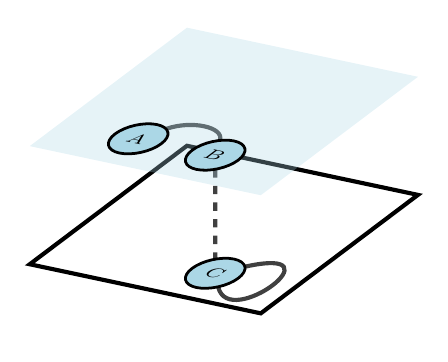
\begin{tikzpicture}[multilayer=3d]
\SetLayerDistance{-1.5}
\Plane[x=-.5,y=-.5,width=3,height=2.5,layer=2,NoFill]
\Plane[x=-.5,y=-.5,width=3,height=2.5,NoBorder]
\Vertex[x=0.5,IdAsLabel,layer=1]{A}
\Vertex[x=1.5,IdAsLabel,layer=1]{B}
\Vertex[x=1.5,IdAsLabel,layer=2]{C}
\Edge[bend=60](A)(B)
\Edge[style=dashed](B)(C)
\Edge(C)(C)
\end{tikzpicture}
\end{document}
%=============================================================================
% eof
%
% Local Variables:
% mode: latex
% mode: linum
% mode: auto-fill
% fill-column: 80
% TeX-master: t
% End:
